%\section{Framework}

The overall structure contains (1) client, (2) server, (3) backend storages.
The structure is shown in Fig.~\ref{fig:frame} 

\begin{figure*}[ht]
\centering
%\includegraphics[width=3.5in]{pics/system_architecture.eps}
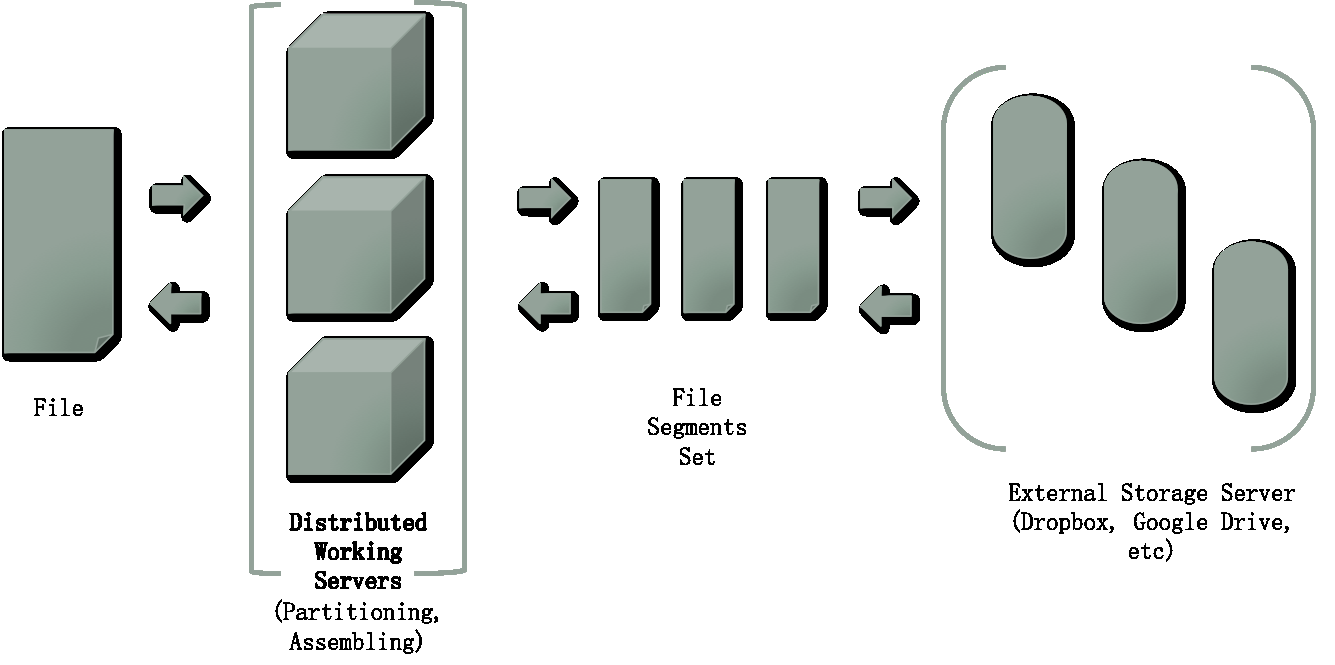
\includegraphics[width=6.5in]{pics/system_architecture-eps-converted-to.pdf}
\caption{Framework}
\label{fig:frame}
\end{figure*}

\subsubsection{Client}
The system (distributed working servers) provide users with uploading, downloading, deleting, newing folders, moving data opeations. Especially for the uploading operation usage, the user is required to set the "black-box" key and specified the security level {normal, high, premium} (higher level means more fragments a file will be partitioned, and it would lead to more time to process), which can be a figure or any combination of string and digits.Besides, the user need give the system access privilege to the external cloud storage servers (Google Drive, SkyDrive, Dropbox, etc). System will automatically maintain a table to record all the files' names and indices of their corresponding partitioned fragments. 

\subsubsection{Server}
Server need be in charge of three responsibilies: determining how to partition the file based on the key given by the user and carrying out the work, communicating with clients and external cloud stroage by transferring kinds of data, assembling the fragments to the original file. In the server, it needs update a dictionary to store which storage server the fragment has been stored and maintains the encrypted version of users' table.
The system still need perform a "heart-beat" function to update this encrypted table by communicating with users periodically.
\subsubsection{External distributed server}
External distrbuted storage servers provide interface to working servers. They are responsible for storing, replicating, backup files.


\section{Software Artifact}
We build a system contains as follows, 

%1. The particular software artifact to complete:

(1) A web interface for user to upload, download files and create folders, etc, like the functionality Dropbox website provides.
When initializing his/her account, the user can choose the security level and integrate with his/her third-party cloud storage platforms.


(2) A server-side distributed files system to handle the file partitioning and assembling, using API from
% Google Drive, 
Dropbox to utilize their services. 
When user uploads a file, our server help partition (or encrypt if the security level is premium) this file, and perform as a \emph{bridge} between
the user and third-party cloud storage server. %to differen 
When user want to fetch a file, it invokes our server-side program to fetch the files fragment from different storage hosts and assemble them into the original file.
The methodology is given in~\ref{sec:approach}.
The blue parts of Fig. \ref{fig:arch} and Fig \ref{fig:web} are built by us.
\begin{comment}
2. A high-level description of the design of your system.

See the section \ref{sec:approach}.

3. Any existing software packages you are using as a basis for your development.

Re-use the Tribble code~\cite{CSE230} with Thrift~\cite{thrift} for interaction with clients (trigger the file transfer), 
Tribble Server (Server in our case, to do the hash and file partitioning, also 
handle the file assembling and respond to users) and 
Backend Storage (invoke API to do the real disk storage). 

We will use the API from Google Drive~\cite{googledriveapi}
and Dropbox~\cite{dropboxapi}.

% We also will use XtremeFS~\cite{xtreemfs} to manage the file partioning and asembling table replication and storage in our server. 

4. Your evaluation plan for this artifact. How will you measure success? What will you use for a testbed? Do you need any resources from us?

For the upload partition of file, in Google Drive and Dropbox, etc, we will dectect the file fragments. When you click the third-party, you cannot see the whole file,
and the third-party cannot recover the file among these unordered fragments.

For fetching a file, the correctness should be gauranteed, it is easy to check to ``diff'' the original file and download file.

The efficiency is the tradeoff with the granularity (security). If user choose large granularity, which will bring more efficiency for partioning or assembling, but less security.
\end{comment}
 
